\documentclass[plain]{article}
\usepackage{lipsum}
\setlength{\oddsidemargin}{0.25 in}
\setlength{\evensidemargin}{-0.25 in}
\setlength{\topmargin}{-0.6 in}
\setlength{\headsep}{0.75 in}
\setlength{\parindent}{0 in}
\textwidth 6.1in
\textheight 9in
\parskip 1ex
\usepackage[framemethod=TikZ]{mdframed}
%
% ADD PACKAGES here:

 \newcommand{\argmax}{\operatornamewithlimits{argmax}}
 \usepackage{todonotes}
\newcommand{\Ex}{\mathbb{E}}
\usepackage{psfrag}
\usepackage{amsmath,amsfonts,graphicx}
\usepackage{amssymb}
\usepackage{tikz}
\usepackage{mathtools}
\usepackage{bbm}
\usepackage{hyperref}
\usepackage{bm}
\usepackage{float}
\usepackage{flexisym}
\usepackage[short]{optidef}
\usepackage{caption}
\usepackage{subcaption}
\usetikzlibrary{shapes,arrows,calc}
\newtheorem{thm}{Theorem}
\newtheorem{example}{Example}
\newtheorem{defin}{Definition}
\newtheorem{defn}{Definition}
\newtheorem{rem}{Remark}
\usepackage{framed}
\newcommand{\Pd}{\mathbb{P}}
\newtheorem{algorithm}{Algorithm}
\newtheorem{fact}{Fact}
\usepackage{natbib}
 \newcounter{lecnum}

\newcommand{\EE}{ \mathsf{E} }
\newcommand{\Var}{ \mbox{Var} }
\newcommand{\Cov}{ \mbox{Cov} }
\newcommand{\1}{\mathbbm{1}}
\newcommand{\Prob}{ \mathsf{P} }
\newcommand{\disfrac}[2]{ {\displaystyle \frac{#1}{#2}} }
\newcommand{\texfrac}[2]{ {\textstyle \frac{#1}{#2}} }
\newcommand{\dissum}[2]{ {\displaystyle \sum_{#1}^{#2}} }
\newcommand{\OR}{ \mbox{~or~} }
\newcommand{\cond}[1]{ \left|\,#1\right. }
\newcommand{\ith}[1]{ #1^{\mbox{\tiny th}} }
\newcommand{\matgen}[1]{ \left[ \begin{array}#1 \end{array} \right] }

\newcommand{\RR}{ {\bf R} }
\newcommand{\NN}{ {\bf N} }
\newcommand{\II}{ {\bf I} }
\newcommand{\ee}{ {\bf e} }
\newcommand{\LL}{ {\bf L} }
\newcommand{\PP}{ {\bf P} }
\newcommand{\calF}{ {\cal F} }
\newcommand{\One}{ \mbox{\sffamily 1} }
\newcommand{\ZZ}{ {\bf Z} }
\newcommand\E{\mathbb{E}}

\newcommand{\R}{{\sf R\hspace*{-0.9ex}%
\rule{0.15ex}{1.5ex}\hspace*{0.9ex}}}
\newcommand{\N}{{\sf N\hspace*{-1.0ex}%
\rule{0.15ex}{1.3ex}\hspace*{1.0ex}}}
\newcommand{\Q}{{\sf Q\hspace*{-1.1ex}%
\rule{0.15ex}{1.5ex}\hspace*{1.1ex}}}
\newcommand{\C}{{\sf C\hspace*{-0.9ex}%
\rule{0.15ex}{1.3ex}\hspace*{0.9ex}}}

\newcommand{\ds}{ \displaystyle }
\bibliographystyle{plain}
%
% The following macro is used to generate the header.
%
\newcommand{\lecture}[4]{
   \pagestyle{myheadings}
   \thispagestyle{plain}
   \newpage
   \noindent
   \begin{center}
   \framebox{
      \vbox{\vspace{2mm}
    \hbox to 6.28in { {\bf Subject}
	\hfill \today} 
       \vspace{4mm}
       \hbox to 6.28in { {\Large \hfill #1  \hfill} }
       \vspace{2mm}
       \hbox to 6.28in { {\hfill \it } }
      \vspace{2mm}
       \hbox to 6.28in { {\hfill \it Author: #2} }
      \vspace{2mm}}
   }
   \end{center}
   \markboth{#1 (#2)}{#1}
   \vspace*{4mm}
}
\usepackage{hyperref}
\usepackage[T1]{fontenc}
\usepackage[utf8]{inputenc}
\usepackage{textcomp} % provide euro and other symbols

\let\b\mathbf

%Use this command for a figure; it puts a figure in wherever you want it.
%usage: \fig{NUMBER}{SPACE-IN-INCHES}{CAPTION}
\newcommand{\fig}[3]{
			\vspace{#2}
			\begin{center}
			Figure \thelecnum.#1:~#3
			\end{center}
	}

\newtheorem{theorem}{Theorem}[lecnum]
\newtheorem{lemma}[theorem]{Lemma}
\newtheorem{proposition}[theorem]{Proposition}
\newtheorem{claim}[theorem]{Claim}
\newtheorem{corollary}[theorem]{Corollary}
\newtheorem{definition}[theorem]{Definition}
\newenvironment{proof}{{\bf Proof:}}{\hfill\rule{2mm}{2mm}}

\begin{document}
\lecture{Notes}{Bryan Tantisujjatham}{1}

\makeatother
\setlength{\emergencystretch}{3em} % prevent overfull lines
\providecommand{\tightlist}{%
  \setlength{\itemsep}{0pt}\setlength{\parskip}{0pt}}
\author{Bryan Tantisujjatham}
\date{\today}

\section{Carbon Free Emissions Plan}
\section{Nationwide Trends}

\section{Current Statistics}


\section{Quantitative Data Analysis}
Population of NYS 19.45 million as of 2019 \cite{noauthor_us_nodate}\\
Population of NYC 8.149 million as of 2019 (cite census)\\

\section{Electricity Demand Forecast}

\subsection{Methods}
\subsection{ARIMA}
\begin{align*}
&y_{t}^{*}=\Delta^{d} y_{t} \\
&y_{t}^{*}=\mu+\underbrace{\sum_{i=1}^{p} \phi_{i} y_{t-i}^{*}}_{\mathrm{AR}}+\underbrace{\sum_{i=1}^{q} \theta_{i} \epsilon_{t-i}+\epsilon_{t}}_{\mathrm{MA}}
\end{align*}
\subsection{Support Vector Regression}
Primal Formulation:
\begin{figure}[H]
	\centering
	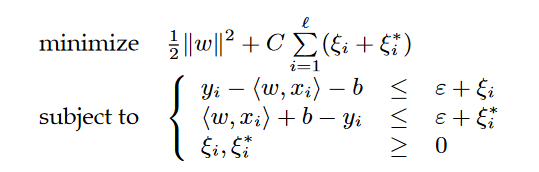
\includegraphics[width=0.5\textwidth]{svm_primal.PNG}
	\caption{}
	\label{fig:}
\end{figure}

Dual Formulation:
\begin{figure}[H]
	\centering
	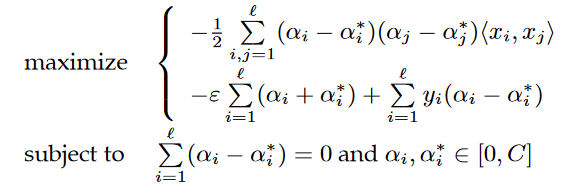
\includegraphics[width=0.5\textwidth]{svm_dual.PNG}
	\caption{}
	\label{fig:}

\end{figure}
\section{Levelized Cost of Energy}
\subsection{LSTM}
\begin{align*}
f_{t} &=\sigma_{g}\left(W_{f} x_{t}+U_{f} c_{t-1}+b_{f}\right) \\
i_{t} &=\sigma_{g}\left(W_{i} x_{t}+U_{i} c_{t-1}+b_{i}\right) \\
o_{t} &=\sigma_{g}\left(W_{o} x_{t}+U_{o} c_{t-1}+b_{o}\right) \\
c_{t} &=f_{t} \circ c_{t-1}+i_{t} \circ \sigma_{c}\left(W_{c} x_{t}+b_{c}\right) \\
h_{t} &=o_{t} \circ \sigma_{h}\left(c_{t}\right)
\end{align*}
\section{New sources of generation}
\subsection{Wind}
\subsubsection{Land}

\subsubsection{Offshore}
New offshore wind projects in pipeline:
\begin{enumerate}
	\item \textbf{Empire Wind 1}: 816 MW, solicited 2018 \cite{noauthor_new_nodate-1}
	\item 	\textbf{Empire Wind 2}: 1260 MW, solicited 2020 \cite{noauthor_new_nodate-1}
	\item \textbf{Sunrise Wind}: 880 MW, solicited 2018 \cite{noauthor_new_nodate-1}
	\item \textbf{Beacon Wind}: 1230 MW, solicited 2020 \cite{noauthor_new_nodate-1}
\end{enumerate}

5 total projects totaling greater than 4300 MW, leading offshore generation pipeline in the nation

Official target goal for offshore wind generation is 9000 MW by 2035. \cite{noauthor_us_nodate-1}

Substation Locations: Astoria Substation, Gowanus Substation, Barrett Substation, Holbrook Substation, East Hampton Substation\\
Proposed Port Facilities: South Brooklyn Marine Terminal, Holbrook Substation, East Hampton Substation. \cite{noauthor_new_nodate-1}

All projects are currently in the data collection phase. \cite{noauthor_new_nodate-1}

NYSERDA offers contracts to purchase offshore renewable energy certificates (OREC) from offshore wind developers. NYSERDA sells these to load serving entities (LSEs) like utilities, which are required by law to purchase renewable energy credits. \cite{NYSERDA_new_nodate-1}

\subsubsection{Technology \& Implementation}
Advances in:
\begin{enumerate}
	\item Materials
	\item Engineering of turbine foudnations
	\item Turbine blade design
\end{enumerate}

With respect to foundations: \cite{mitchell_review_2022}
\begin{enumerate}
	\item Monopiles - for depths up to 25m. Freestanding; cheap, easy to install and inexpensive to manufacture and transport. Used in 95\& of installations worldwide.
	\item Gravity - also for up to 25m, but used for les cohesive seabed compositions
	\item Suction bucket - Can also be cost effective, but oly for appropriate choice of seabed composition
	\item Deepwater - 
	\item Tripod - 30m - 60m water depth
	\item Jacket - > 50m water depth. Expensive and complex to install and manufacture; however, mature
\end{enumerate}
\subsubsection{Geography of the Long-Island Area}

\subsection{Solar}
Official target: 10GW distributed solar by 2030 (cite NYSERDA)\\
Government sponsored incentives via tax credits, NYSun

\subsection{Geothermal}
\section{Maintenance of mature technologies and infrastructure}
\subsection{Nuclear}



\section{Policy Changes}
NYSERDA energy credits:
	\begin{enumerate}
		\item Tier 1 (new renewables)
		\item Tier 2 (maintenance resources)
		\item Tier 2 (competitive program)
		\item Tier 4 (NYC renewable energy)
	\end{enumerate}
\subsection{Pricing Changes}
\subsection{Economic viability}
Need Fair distribution of costs between ISOs and RTOs. \cite{mitchell_review_2022}\\
Renewable Portfolio Standards\\
Aggressive federal support amenable to policy decision to focus on offshore wind -- allows ISOs to reach LCOE  levels for offshore installation costs similar to those seen in the UK, given the tax subsidies \cite{mitchell_review_2022}\\

\section{Viability (outside of financial)}
\subsection{Resource constraints}
\subsection{Trend constraints}
\subsection{Location constraints}
\section{Background}
The last two decades have brought marked improvements in energy efficient systems and infrastructure on a global scale. The penetration profile of electricity generation sources has seen a nationwide trend towards renewable and "clean" energy source -- offshore wind, nuclear, biofuels, and geothermal -- and a complementary shift away from traditional fossil fuels. 

The NYISO region is uniquely characterized by the speed at which it has adopted -- and integrated -- new technologies and developed infrastructure. It remains the only coal free region in the US, and leads the nation in installed capacity of several renewable sources -- most notably offshore wind [cite NYSERDA]. With five offshore wind projects in active development, New York is touted as the nation's "hub" for offshore wind, projecting to deliver approximately 4300 MW from these facilities alone, with goals to extend that to 9000 MW by 2040 \todo{citation}. Quite remarkably, New York consumes less total energy per capita than all but two states, and \todo{a little more here?}.

While the NYISO has released a comprehensive plan towards 70\% renewable energy by 2030, and 100\% carbon-free electricity by 2040, 
there are several areas which remain unexploited. Our work aims to assess these areas of untapped potential and improvements in policy that can be leveraged to accelerate progress towards this goal. We also provide a robust, quantitative analysis of projected energy demand and projected generation requirements needed to sustain this trend towards 100\% carbon-free electricity in the next eight years.

\subsection{Statewide Energy Profile}
New York has consistently met nearly 90\% of energy requirements through nuclear, hydropower and natural gas alone. [citation]
\subsection{Technology}

\subsection{Policy}
\subsubsection{NYSUN}
\begin{enumerate}
	\item NYSun PV
\end{enumerate}
\subsubsection{Tax Credits and Subsidies}
\begin{enumerate}
	\item Solar Energy System Equipment Credits
	\item OREC for offshore wind solicitatoins
	\item 
\end{enumerate}

\subsection{Infrastructure}

\subsection{Control}
Recent innovations in in statistical modeling, in particular data-driven optimization and machine learning, have severely overhauled the standard procedures for management of electricity on the grid. 

Interst in smart-buildings and online optimization techniques for realtime energy usage has exploded \cite{yu_review_2021}, \cite{khan_modeling_2022}, \cite{sembroiz_planning_2019}, especially with the advent of reinforcement learning and robust model predictive control \cite{chen_efficient_2020}, \cite{yang_adaptive_2019}. \todo{more RL citations}. 

\section{Main points (for slide)}

\bibliography{cite}
\end{document}
